% Created 2015-02-12 Thu 13:24
\documentclass[11pt]{article}
\usepackage[utf8]{inputenc}
\usepackage[T1]{fontenc}
\usepackage{fixltx2e}
\usepackage{graphicx}
\usepackage{longtable}
\usepackage{float}
\usepackage{wrapfig}
\usepackage{soul}
\usepackage{textcomp}
\usepackage{marvosym}
\usepackage{wasysym}
\usepackage{latexsym}
\usepackage{amssymb}
\usepackage{hyperref}
\tolerance=1000
\usepackage{methodshw}
\usepackage{booktabs}
\providecommand{\alert}[1]{\textbf{#1}}

\title{8004 Homework 2}
\author{Nooreen Dabbish}
\date{\today}
\hypersetup{
  pdfkeywords={},
  pdfsubject={},
  pdfcreator={Emacs Org-mode version 7.9.3f}}

\begin{document}

\maketitle


\section{Suppose that we are working under the Gauss-Markov model}
\label{sec-1}

\[ \mathbf{Y} = \mathbf{X\beta} + \mathbf{\epsilon} \]
where $E(\epsilon) = \mathbf{0}$ and
$var(\epsilon)=\sigma^2\mathbf{I}$. Let $\hat{\mathbf{Y}}$ be the
ordinary least square estimator of $\mathbf{Y}$.
 
\subsection{Show that $\hat{\mathbf{Y}}$ and $\mathbf{Y} - \hat{\mathbf{Y}}$ are uncorrelated.}
\label{sec-1-1}


Let $\hat{\mathbf{Y}} = P_X Y = X(X'X)^{-}X'Y$.

First, note that $\hat{\mathbf{Y}}$ and $\mathbf{Y} -
\hat{\mathbf{Y}}$ are orthogonal.

\[
\hat{\mathbf{Y}}'(\mathbf{Y} - \hat{\mathbf{Y}}) = (\mathbf{P_X Y})'(\mathbf{Y} - \mathbf{P_x Y})\\
                                                 = \mathbf{Y}'
                                                 \mathbf{P_X}' (\mathbf{Y} -
                                                 \mathbf{P_x Y})\\
                                                 =
                                                 \mathbf{Y}'\mathbf{P_X
                                                 Y} -
                                                 \mathbf{Y}'\mathbf{P_X}'\mathbf{P_X
                                                 Y}\\
                                                 =
                                                 \mathbf{Y}'\mathbf{P_X}\mathbf{Y} -
                                                 \mathbf{Y}'\mathbf{P_X}\mathbf{Y}\\
                                                 =\mathbf{0}
\]

Therefore, the expectation 
\[
E(\hat{\mathbf{Y}}'(\mathbf{Y} -
\hat{\mathbf{Y}}))=E(\mathbf{0})=\mathbf{0}
\]

\[
E(\hat{\mathbf{Y}})=E(\mathbf{X\hat{\beta}})\\
                   =X E(\hat{\beta})\\
                   =X\beta
\]

\[
E(\mathbf{Y} - \hat{\mathbf{Y}})= \mathbf{X\beta} - \mathbf{X\beta} \\
                                = \mathbf{0}
\]

This shows $\hat{\mathbf{Y}}$ and $\mathbf{Y} - \hat{\mathbf{Y}}$ are
uncorrelated because $E(\hat{\mathbf{Y}}(\mathbf{Y} -
\hat{\mathbf{Y}}) - E(\hat{\mathbf{Y}})E(\mathbf{Y} -
\hat{\mathbf{Y}})$ is zero.
\subsection{Show that}
\label{sec-1-2}

$$ E\{(\mathbf{Y} - \hat{\mathbf{Y}})^T(\mathbf{Y} -
\hat{\mathbf{Y}})\} = \sigma^2\{n-\mathrm{rank}(\mathbf{X})\}.$$
You may use Theorem 5.2a of R\&S.


Theorem 5.2a states:
If \textbf{y} is a random vector with mean \textbf{$\mu$} and covariance
matrix \textbf{$\Sigma$} and if \textbf{A} is a symmetric matrix of contants, then 
\[
E(\mathbf{y'Ay}) = tr(\mathbf{A\Sigma}) +\mathbf{\mu' A \mu}.
\]


We can apply Theorem 5.2a with \textbf{A} = \textbf{I} and $\mathbf{y} =
\mathbf{Y} - \hat{\mathbf{Y}}$. From part a) above, our mean \textbf{$\mu$}
is \textbf{0}. The term $\mathbf{\mu' A \mu}$ is therefore \textbf{0}, and the
expression of interest becomes:

$$E\{(\mathbf{Y} - \hat{\mathbf{Y}})^T(\mathbf{Y}
-\hat{\mathbf{Y}})\}   = tr(\Sigma)$$

Where $\Sigma$ is the covariance matrix of $\mathbf{Y} - \hat{\mathbf{Y}}$.

\begin{align*}
Var(\mathbf{Y} - \hat{\mathbf{Y}}) &= Var ((\mathbf{I} - \mathbf{P_X})Y) \\
&= (\mathbf{I} - \mathbf{P_X}) Var(Y) (\mathbf{I} - \mathbf{P_X})' \\
&= (\mathbf{I} - \mathbf{P_X}) Var(Y) (\mathbf{I} - \mathbf{P_X}) \\
&= (\mathbf{I} - \mathbf{P_X}) \sigma^2 \mathbf{I} (\mathbf{I} - \mathbf{P_X}) \\
&= \sigma^2(\mathbf{I} - \mathbf{P_X})
\end{align*}

Trace of $\mathbf{I} - \mathbf{P_X}$ is
$tr(\mathbf{I})-tr(\mathbf{P_X})$. 
The trace of an \emph{nxn} identity matrix \textbf{I} is n, and the trace a
projection matrix is the rank of target space, $tr(P_X) = rank(X)$.
The trace of product of a scalar \emph{c} and a matrix \textbf{A} is the product
$tr(c\mathbf{A}) = c tr(\mathbf{A})$. Thus, $tr(\sigma^2(\mathbf{I} -
\mathbf{P_X})) = \sigma^2 (n - \mathrm{rank}(\mathbf{X}))$.
This gives the desired result: 
$$ E\{(\mathbf{Y} - \hat{\mathbf{Y}})^T(\mathbf{Y} -\hat{\mathbf{Y}})\} 
= \sigma^2\{n-\mathrm{rank}(\mathbf{X})\}.$$
\section{Consider the one-way ANOVA model $y_{ij} = \mu + \tau_i + \epsilon_{ij}$ for the jth individual of the ith group .}
\label{sec-2}

Suppose there are 4 treatments (groups) and the sample sizes are 
respectively 2,1,1,2 for treatments.
Now suppose that $\mathbf{Y} = (y_{11}, y_{12}, y_{21}, y_{31},
y_{41}, y_{42})^{T} = (2, 1, 4, 6, 3, 5)^{T}$ contains the observations.

Use R and weighted generalized least squares to find an appropriate 
estimate for
$$E(\mathbf{Y})\,\mathrm{and}\,
\begin{pmatrix}
1 & 1 & 0 & 0 & 0 \\
1 & 0 & 1 & 0 & 0 \\
1 & 0 & 0 & 1 & 0 \\
1 & 0 & 0 & 0 & 1 
\end{pmatrix}\mathbf{\beta}$$
in the Aiken model with $\mathrm{var}(\epsilon) = \mathbf{V}$ for two
cases where
 
\subsection{$\mathbf{V} = \mathbf{V}_1 = \mathrm{diag}(1,9,9,1,1,9)$}
\label{sec-2-1}



The full model described in this question in 
$\mathbf{Y}=\mathbf{X\beta}+\epsilon$ matrix form is:

\[
\begin{pmatrix}
y_{11} \\ y_{12}\\ y_{21}\\ y_{31}\\ y_{41}\\ y_{42}
\end{pmatrix} = 
\begin{pmatrix} 
2\\ 1\\ 4\\ 6\\ 3\\ 5
\end{pmatrix} = 
\begin{pmatrix}
1 & 1 & 0 & 0 & 0 \\
1 & 1 & 0 & 0 & 0 \\
1 & 0 & 1 & 0 & 0 \\
1 & 0 & 0 & 1 & 0 \\
1 & 0 & 0 & 0 & 1 \\
1 & 0 & 0 & 0 & 1 \\
\end{pmatrix}  
\begin{pmatrix}
\mu \\ \tau_1 \\ \tau_2 \\ \tau_3 \\ \tau_4 
\end{pmatrix} + 
\begin{pmatrix}
\epsilon_{11} \\ \epsilon_{12}\\ \epsilon_{21}\\ \epsilon_{31}\\ \epsilon_{41}\\ \epsilon_{42}
\end{pmatrix}
\]

We have $var(\epsilon) = \sigma^2 \mathbf{V}$, so we must re-write
the model in terms of $\mathbf{U} = \mathbf{V}^{-1/2}\mathbf{Y}$ as
follows:

\begin{align*}
\mathbf{V} &= \mathbf{V}^{1/2} \mathbf{V}^{1/2},\, \text{V is a
diagonal matrix}\\
\mathrm{Let }\, \mathbf{U}& =\mathbf{V}^{-1/2}Y\\ E(\mathbf{U}) &= \mathbf{V}^{-1/2}E{Y} = \mathbf{V}^{-1/2}\mathbf{X\beta}\\
&= \mathbf{W\beta}\\
Var(\mathbf{U}) &= \mathbf{V}^{-1/2} Var(\mathbf{Y})\mathbf{V}^{-1/2}\\
                &= \sigma^2 \mathbf{V}^{-1/2} \mathbf{V}\mathbf{V}^{-1/2}\\
                &= \sigma^2 \mathbf{I}\\
\epsilon^{\star} &= \mathbf{V}^{-1/2} \mathbf{\epsilon}\\
E(\epsilon^{\star}) &= E(\mathbf{V}^{-1/2}\epsilon) \\
                    &= \mathbf{V}^{-1/2}E(\epsilon) \\
                    &= \mathbf{0}\\
Var(\epsilon^{\star}) &= Var(\mathbf{V}^{-1/2}\epsilon) \\
                      &= \mathbf{V}^{-1/2} Var(\epsilon) \mathbf{V}^{-1/2}\\
                      &= \mathbf{V}^{-1/2} \sigma^2 \mathbf{V} \mathbf{V}^{-1/2}\\
                      &= \sigma^2 \mathbf{I}
\end{align*}

This gives us $\mathbf{U} = \mathbf{W\beta} + \epsilon^{\star}$, where
the Gauss-Markov assumptions hold for \textbf{U}.

We first calculate \textbf{V$^{\mathrm{-1/2}}$}:

\begin{align*}
\mathbf{V} &= \mathbf{V}_1 = \mathrm{diag}(1,9,9,1,1,9)\\
\text{So,}\, \mathbf{V}^{1/2}_1 &= \mathrm{diag}(1,3,3,1,1,3)\\
             \mathbf{V}^{-1/2}_1 &= \mathrm{diag}(1,1/3,1/3,1,1,1/3)\\
\end{align*}

We can check this in R,

\begin{verbatim}
V <- diag(c(1,9,9,1,1,9))
Vhi <- solve(V^(1/2))
lvector(Vhi)
\end{verbatim}

\[
\mathbf{V}^{-1/2} = 
% latex table generated in R 3.0.2 by xtable 1.7-4 package
% Tue Feb 10 14:46:43 2015
\begin{pmatrix}{}
  1.00 & 0.00 & 0.00 & 0.00 & 0.00 & 0.00 \\ 
  0.00 & 0.33 & 0.00 & 0.00 & 0.00 & 0.00 \\ 
  0.00 & 0.00 & 0.33 & 0.00 & 0.00 & 0.00 \\ 
  0.00 & 0.00 & 0.00 & 1.00 & 0.00 & 0.00 \\ 
  0.00 & 0.00 & 0.00 & 0.00 & 1.00 & 0.00 \\ 
  0.00 & 0.00 & 0.00 & 0.00 & 0.00 & 0.33 \\ 
  \end{pmatrix}
\]

\begin{align*}
\mathbf{U} &= \mathbf{V}^{-1/2} \mathbf{Y} = 
\begin{pmatrix}
y_{11} \\ \frac{1}{3} y_{12}\\ \frac{1}{3} y_{21}\\ y_{31}\\ y_{41}\\ \frac{1}{3}y_{42}
\end{pmatrix} = 
\begin{pmatrix} 
2\\ \frac{1}{3}\\ \frac{4}{3}\\ 6\\ 3\\ \frac{5}{3}
\end{pmatrix}
\end{align*}

Checking \textbf{U} in R gives:

\begin{verbatim}
Y <- matrix(c(2, 1, 4, 6, 3, 5), nrow=6, ncol=1)
U <- Vhi %*% Y
lvector(U)
\end{verbatim}

\[
\mathbf{U} =
% latex table generated in R 3.0.2 by xtable 1.7-4 package
% Wed Feb 11 19:13:05 2015
\begin{pmatrix}{}
  2.00 \\ 
  0.33 \\ 
  1.33 \\ 
  6.00 \\ 
  3.00 \\ 
  1.67 \\ 
  \end{pmatrix}
\]

\begin{align*}
\mathbf{W} &= \mathbf{V}^{-1/2}\mathbf{X} \\
           &= \mathrm{diag}(1,1/3,1/3,1,1,1/3)\begin{pmatrix}
1 & 1 & 0 & 0 & 0 \\
1 & 1 & 0 & 0 & 0 \\
1 & 0 & 1 & 0 & 0 \\
1 & 0 & 0 & 1 & 0 \\
1 & 0 & 0 & 0 & 1 \\
1 & 0 & 0 & 0 & 1 
\end{pmatrix}  \\
 &= 
\begin{pmatrix}{}
  1           & 1           & 0           & 0 & 0 \\
  \frac{1}{3} & \frac{1}{3} & 0           & 0 & 0 \\
  \frac{1}{3} & 0           & \frac{1}{3} & 0 & 0 \\
  1           & 0           & 0           & 1 & 0 \\
  1           & 0           & 0           & 0 & 1 \\
  \frac{1}{3} & 0           & 0           & 0 & \frac{1}{3} 
  \end{pmatrix}
\end{align*}

Checking \textbf{W} in R gives:

\begin{verbatim}
X <- matrix(c(rep(1,6),
              1,1,0,0,0,0,
              0,0,1,0,0,0,
              0,0,0,1,0,0,
              0,0,0,0,1,1),nrow = 6,byrow=FALSE)
W <- Vhi %*% X
lvector(W)
\end{verbatim}

\[
\mathbf{W} =
% latex table generated in R 3.0.2 by xtable 1.7-4 package
% Wed Feb 11 22:05:45 2015
\begin{pmatrix}{}
  1.00 & 1.00 & 0.00 & 0.00 & 0.00 \\ 
  0.33 & 0.33 & 0.00 & 0.00 & 0.00 \\ 
  0.33 & 0.00 & 0.33 & 0.00 & 0.00 \\ 
  1.00 & 0.00 & 0.00 & 1.00 & 0.00 \\ 
  1.00 & 0.00 & 0.00 & 0.00 & 1.00 \\ 
  0.33 & 0.00 & 0.00 & 0.00 & 0.33 \\ 
  \end{pmatrix}
\]
\subsubsection{Solving for $\hat{E(Y)}$: $\mathbf{U} = \mathbf{W\beta} + \mathbf{\epsilon}$ for $\hat{\mathbf{U}}$}
\label{sec-2-1-1}


\begin{align*}
\hat{\mathbf{U}} &=
\mathbf{W}(\mathbf{W}'\mathbf{W})^{-}\mathbf{W}'\mathbf{Y}
\end{align*}

\begin{verbatim}
Uhat <- W %*% ginv(t(W) %*% W) %*% t(W) %*% U
lvector(Uhat)
\end{verbatim}

\[
\hat{\mathbf{U}} =
% latex table generated in R 3.0.2 by xtable 1.7-4 package
% Wed Feb 11 22:11:29 2015
\begin{pmatrix}{}
  1.90 \\ 
  0.63 \\ 
  1.33 \\ 
  6.00 \\ 
  3.20 \\ 
  1.07 \\ 
  \end{pmatrix}
\]

Now, we can solve for $\hat{E(\mathbf{Y})} = \hat{\mathbf{Y}} =
\mathbf{V}^{1/2}\hat{\mathbf{U}}$:


\begin{verbatim}
Yhat <- (V^{1/2})%*%Uhat
lvector(Yhat)
\end{verbatim}

\[
\hat{E(\mathbf{Y})} =
% latex table generated in R 3.0.2 by xtable 1.7-4 package
% Wed Feb 11 22:16:51 2015
\begin{pmatrix}{}
  1.90 \\ 
  1.90 \\ 
  4.00 \\ 
  6.00 \\ 
  3.20 \\ 
  3.20 \\ 
  \end{pmatrix}
\]
\subsubsection{Solving for $\hat{\mathbf{C}'\beta}$ given by:}
\label{sec-2-1-2}


\[
\begin{pmatrix}
1 & 1 & 0 & 0 & 0 \\
1 & 0 & 1 & 0 & 0 \\
1 & 0 & 0 & 1 & 0 \\
1 & 0 & 0 & 0 & 1 
\end{pmatrix}\mathbf{\beta}
\]

We have $\hat{\mathbf{C'\beta}}(\mathbf{U}) = \mathbf{C}'(\mathbf{W}'\mathbf{W})^{-}\mathbf{W}'\mathbf{U}$


\begin{verbatim}
CT <- matrix(c(1,1,0,0,0,1,0,1,0,0,1,0,0,1,0,1,0,0,0,1), nrow=4,ncol=5, byrow=T)
CTBetahat <- CT %*% ginv(t(W)%*%W) %*% t(W) %*% U
lvector(CTBetahat)
\end{verbatim}

\[
\hat{\mathbf{C}'\mathbf{\beta}} =
% latex table generated in R 3.0.2 by xtable 1.7-4 package
% Wed Feb 11 22:43:35 2015
\begin{pmatrix}{}
  1.90 \\ 
  4.00 \\ 
  6.00 \\ 
  3.20 \\ 
  \end{pmatrix} =
\begin{pmatrix}
\widehat{\mu + \tau_1} \\
\widehat{\mu + \tau_2} \\
\widehat{\mu + \tau_3} \\
\widehat{\mu + \tau_4}
\end{pmatrix}
\]
\subsection{V$_2$}
\label{sec-2-2}

\[ 
\mathbf{V} = \mathbf{V}_2 = 
\begin{pmatrix}
1 & 1 & 0 & 0 & 0 & 0 \\
1 & 9 & 0 & 0 & 0 & 0 \\
0 & 0 & 9 & -1& 0 & 0 \\
0 & 0 & -1& 1 & 0 & 0 \\
0 & 0 & 0 & 0 & 1 & -1 \\
0 & 0 & 0 & 0 & -1 & 9
\end{pmatrix}
\]
\subsubsection{Tranformation to OLS using \textbf{V$^{\mathrm{-1/2}}$}}
\label{sec-2-2-1}


The a square root matrix $\mathbf{V_2}^{1/2}$ can be found as follows:

\begin{itemize}
\item Write a matrix \textbf{D$^{\mathrm{1/2}}$} containing the square root's of \textbf{V$_2$}'s eigenvalues in its' diagonal.
\item Write a matrix \textbf{C} whose columns are the normalized eigenvectors of \textbf{V$_2$}.
\item \textbf{V$_2$$^{\mathrm{1/2}}$} is the product $\mathbf{CD^{1/2}C'}$.
\end{itemize}

We will use the square root as above to transform the GLS equations
into OLS as above.
     

\begin{verbatim}
Dh <- diag(sqrt(eigen(V)$values))
C <- eigen(V)$vectors 
Vh <- C %*% Dh %*% t(C)
Vhi <- solve(Vh)

Y <- matrix(c(2, 1, 4, 6, 3, 5), nrow=6, ncol=1)
Yp <- Vhi %*% Y

X <- matrix(c(rep(1,6),
              1,1,0,0,0,0,
              0,0,1,0,0,0,
              0,0,0,1,0,0,
              0,0,0,0,1,1),nrow = 6,byrow=FALSE)
Xp <- Vhi %*% X


Yphat <- Xp %*% ginv(t(Xp) %*% Xp) %*% t(Xp) %*% Yp
Yhat <- (Vh)%*%Yphat
lvector(Yhat)

CT <- matrix(c(1,1,0,0,0,1,0,1,0,0,1,0,0,1,0,1,0,0,0,1), nrow=4,ncol=5, byrow=T)
CTBetahat <- CT %*% ginv(t(Xp)%*%Xp) %*% t(Xp) %*% Yp
lvector(CTBetahat)
\end{verbatim}

Results obtained for $\widehat{E(\mathbf{Y})}$ and \$\widehat{C'\beta}* are:

\[
\widehat{E(\mathbf{Y})} =
\begin{pmatrix}{}
  2.00 \\ 
  2.00 \\ 
  4.00 \\ 
  6.00 \\ 
  3.33 \\ 
  3.33 \\ 
  \end{pmatrix}\,\,\mathrm{and}\,\,\widehat{\mathbf{C'\beta}} =
\begin{pmatrix}{}
  2.00 \\ 
  4.00 \\ 
  6.00 \\ 
  3.33 \\ 
  \end{pmatrix}
\]
\section{The lm function in R allows one to do weighted least squares}
\label{sec-3}

 with the form $\sum w_i(y_i-\hat{y}_i)^2$ for positive weights $w_i$.
 For $\mathbf{V}_1$ in the last question, find the BLUEs of the 4 cell
 means using lm and an appropriate vector of weights.


I call lm to model $\mathbf{Y}$ as a function of the design matrix $\mathbf{X}$ with
``no intercept'' and with the weights from the diagonal of $\mathbf{V_1}^{-1}$.


\begin{verbatim}
V <- diag(c(1,9,9,1,1,9))
Y <- matrix(c(2, 1, 4, 6, 3, 5), nrow=6, ncol=1)
X <- matrix(c(rep(1,6),
              1,1,0,0,0,0,
              0,0,1,0,0,0,
              0,0,0,1,0,0,
              0,0,0,0,1,1),nrow = 6,byrow=FALSE)
lmod <- lm(Y ~ 0 + X[,2:5], weights=diag(solve(V)))
xtable(summary(lmod))
\end{verbatim}

\begin{table}[ht]
\centering
Results of calling lm with weights from $V_1^{-1}$\\
\begin{tabular}{rrrrrr}
  \hline
 Parameter & X-location & Estimate & Std. Error & t value & Pr(>|t|) \\ 
  \hline
$\widehat{\mu + \tau_1}$ & X[, 2:5]1 & 1.9000 & 0.4743 & 4.01 & 0.0570 \\ 
$\widehat{\mu + \tau_2}$ &  X[, 2:5]2 & 4.0000 & 1.5000 & 2.67 & 0.1165 \\ 
$\widehat{\mu + \tau_3}$ &  X[, 2:5]3 & 6.0000 & 0.5000 & 12.00 & 0.0069 \\ 
$\widehat{\mu + \tau_4}$ &  X[, 2:5]4 & 3.2000 & 0.4743 & 6.75 & 0.0213 \\ 
   \hline
\end{tabular}
\end{table}

The parameter estimates generated here by \verb~lm~ are idetical to those obtained in
question 2a, using \textbf{V$_1$} as a source of weights.
\section{By running}
\label{sec-4}



\begin{verbatim}
library(MASS)
data(Boston)
\end{verbatim}

will load the Boston housing data into R. Use \verb~?Boston~ to see the
information on the variables. Now create two matrixes $\mathbf{Y}$
and $\mathbf{X}$ that will be used to fit a regression model to some
of these data.

\rule{0.5\textwidth}{0.5pt}

Information on the variables:

\begin{verbatim}
?Boston
\end{verbatim}



\begin{verbatim}
Y=as.matrix(Boston$medv)
X=as.matrix(Boston[,c('crim','nox','rm','age','dis')])
X=cbind(rep(1,dim(Boston)[1]),X)
\end{verbatim}
\subsection{Make a scatterplot matrix for $y,x_1,\ldots,x_5$.}
\label{sec-4-1}

If you had to guess based on this plot, which single predictor 
do you think is probably the best predictor of Price? Do you 
see any evidence of multicollinearity (correlation among the
predictors) in this graphic?


\begin{verbatim}
myscatter <- data.frame(cbind(Y,X[,c(2:6)]))
plot(myscatter)
\end{verbatim}

\begin{figure}[H]
\centering
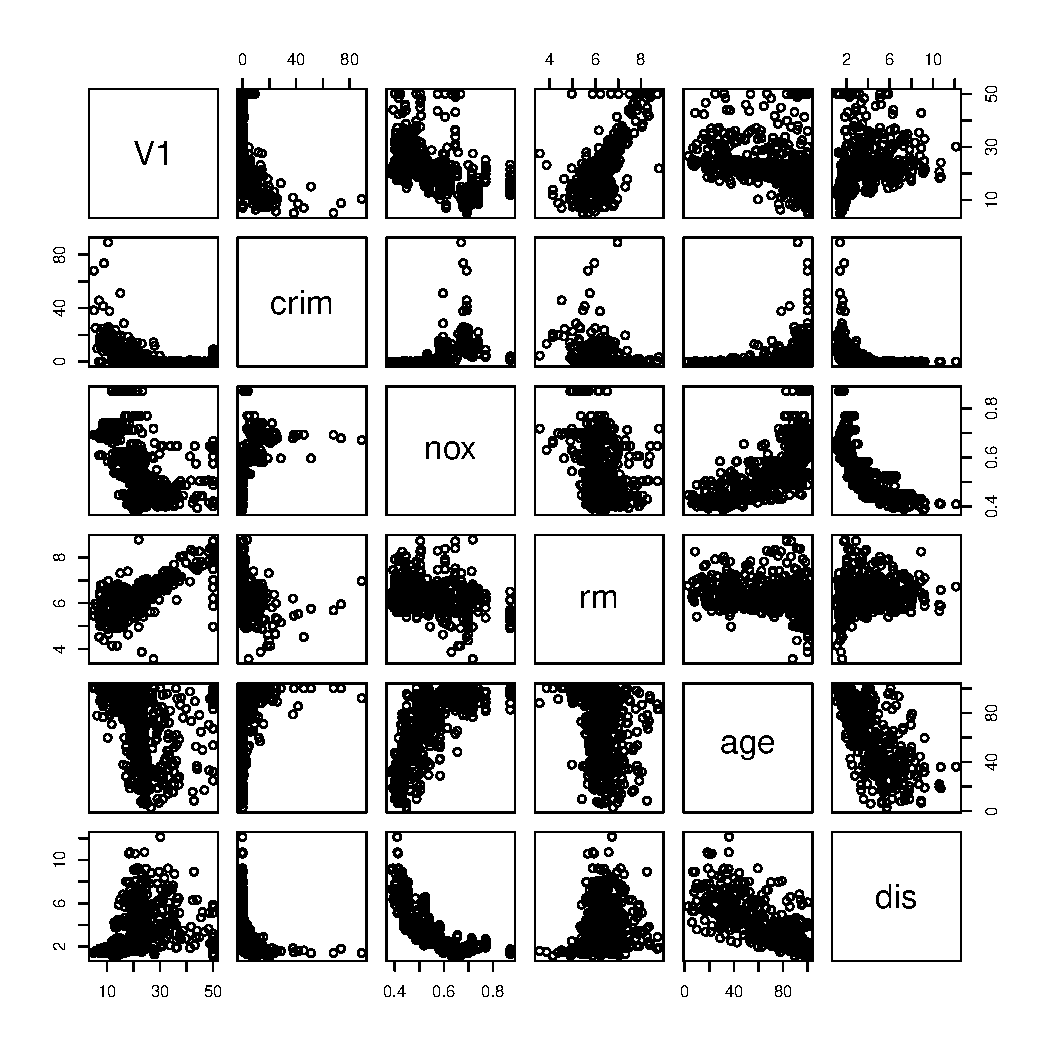
\includegraphics[width=0.7\textwidth]{HW2_4a.pdf}
\caption{Scatterplot matrix showing relationships amoung Boston housing data variables.}
\end{figure}

Based on this scatterplot, I think that `rm' the average number of
rooms per dwelling is the best predictor of price, `V1'. There is
strong evidence of multicollinearity in the scatter
plot. The ‘age’ or fraction of owner-occupied units built prior to
1940 and `dis' the weighted mean of distances to five Boston 
employment centres appear to have a strong linear relationship, as
`age' increases, `dis' tends to decrease. `nox', the concentration of
Nitrous Oxide has a linear relationship with `age' as well as `dis'.
\subsection{Use qr() function to find the rank of \textbf{X}}
\label{sec-4-2}



\begin{verbatim}
qr(X)$rank
\end{verbatim}

The rank of $\mathbf{X}$ is 6.
\subsection{Use R matrix operations on the $\mathbf{X}$ matrix and $\mathbf{Y}$ vector}
\label{sec-4-3}

to find the estimated coefficient vector $\hat{\beta}$, the estimated
mean vector $\hat{\mathbf{Y}}$, and the vector of residuals
$\mathbf{e} = \mathbf{Y} - \mathbf{\hat{Y}}$.

\[ \hat{\beta} = (\mathbf{X}'\mathbf{X})^{-}\mathbf{X}'\mathbf{Y} \]


\begin{verbatim}
betahat <- ginv(t(X)%*%X) %*% t(X) %*% Y
lvector(betahat)
\end{verbatim}

\[
\hat{\beta} =
\begin{pmatrix}{}
  -6.23 \\ 
  -0.21 \\ 
  -18.05 \\ 
  7.74 \\ 
  -0.07 \\ 
  -1.19 \\ 
  \end{pmatrix}
\]

\[ \hat{\mathbf{Y}} = \mathbf{X} (\mathbf{X}'\mathbf{X})^{-}\mathbf{X}'\mathbf{Y} \]
Also, $\hat{\mathbf{Y}} = \mathbf{X}\hat{\beta}$.


\begin{verbatim}
Yhat <- X %*% betahat
err <- Y- Yhat
lvector(Yhat)
lvector(err)
\end{verbatim}

\[
\mathbf{\hat{Y}} =
\begin{pmatrix}{}
  25.70 \\ 
  23.80 \\ 
  30.89 \\ 
  \vdots \\
  28.73 \\ 
  27.17 \\ 
  21.70 \\ 
  \end{pmatrix},\,\,\,\text{and}\,\,\mathbf{e} =
\begin{pmatrix}{}
  -1.70 \\ 
  -2.20 \\ 
  3.81 \\ 
   \vdots \\
  -4.83 \\ 
  -5.17 \\ 
  -9.80 \\ 
  \end{pmatrix}
\]
\subsection{Plot the residuals against the fitted means}
\label{sec-4-4}



\begin{verbatim}
plot(Yhat, err, xlab="Yhat, Fitted Means", ylab="Y-Yhat, Residuals")
\end{verbatim}

\begin{figure}[H]
\centering
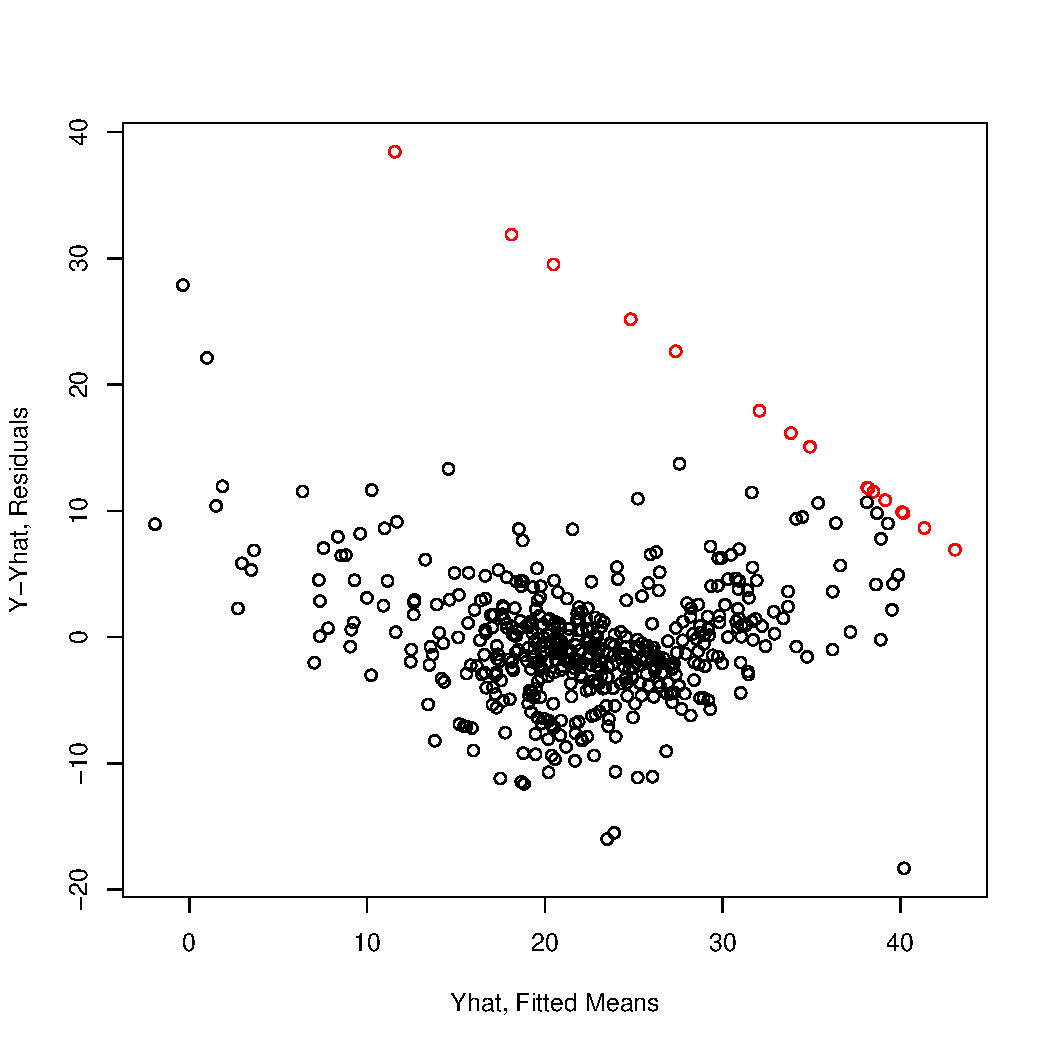
\includegraphics[width=0.7\textwidth]{HW2_4d.pdf}
\caption{Residuals versus fitted means.}
\end{figure}


In this plot, there does seem to be non-constant variance,
heteroscedasticity, which is perhaps nonlinear. The residuals 
tend to be farthest from zero for the smallest and largest Yhat
values.

There is also some kind of artifact creating a straight line in 
upper right hand corner of the graph. 
\subsection{Create a normal plot from the values in the residuals vector.}
\label{sec-4-5}


This plot asseses the residuals for normality. I used the \verb~qqnorm~
and \verb~qqline~ functions. 


\begin{verbatim}
qqnorm(err, ylab="Residuals", main="Normal Q-Q plot for Boston Housing Data Residuals")
qqline(err)
\end{verbatim}

\begin{figure}[H]
\centering
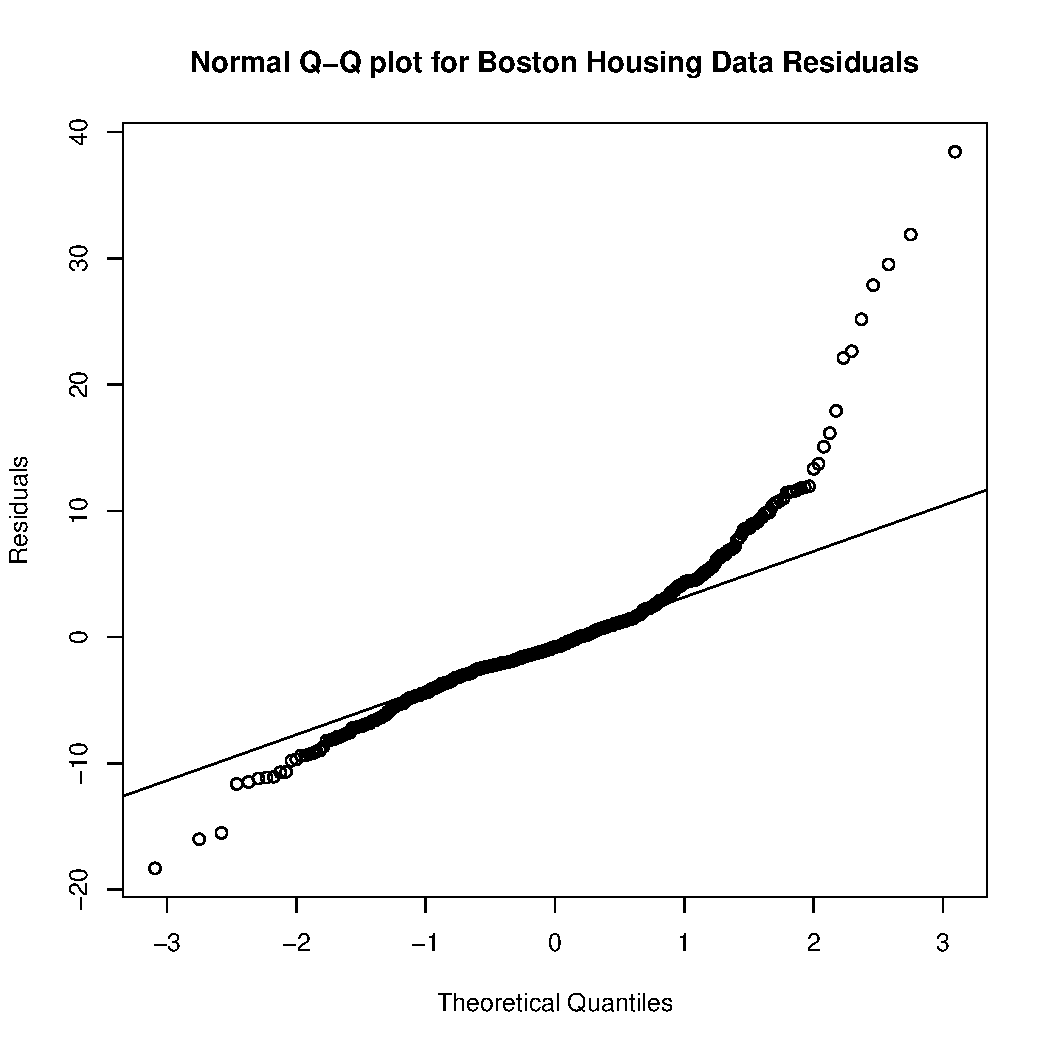
\includegraphics[width=0.7\textwidth]{HW2_4e.pdf}
\caption{Normal Q-Q Plot for Boston Housing data.}
\end{figure}
\subsection{Compute the sum of squared residulas and the corresponding estimates of $\sigma$$^2$}
\label{sec-4-6}


\[ \hat{\sigma^2} =
\frac{(\mathbf{Y}-\hat{\mathbf{Y}})'(\mathbf{Y}-\hat{\mathbf{Y}})}{n -
\text{rank}(\mathbf{X})}
\]


\begin{verbatim}
sigsqhat <- t(err) %*% err / (dim(X)[1] - qr(X)$rank)
sigsqhat
\end{verbatim}

The estimate obtained for $\hat{\sigma^2}$ was 34.82387.
\subsection{Call the lm function in R and confirm your answers,}
\label{sec-4-7}

and note that \verb~?lm~ gives you various information such as the outputs
of the function.


\begin{verbatim}
ml = lm(medv~crim+nox+rm+age+dis, data=Boston)
summary(ml)
xtable(summary(ml))
\end{verbatim}


Call:
lm(formula = medv \~{} crim + nox + rm + age + dis, data = Boston)

\begin{table}[ht]
\centering
Residuals:\\
\begin{tabular}{rrrrr}
\hline
    Min   &   1Q &   Median &      3Q  &     Max\\
\hline 
-18.313  & -2.917 &  -0.785 &   1.979 &  38.442 \\
\hline
\end{tabular}
\end{table}

\begin{table}[ht]
\centering
Coefficients:\\
\begin{tabular}{rrrrr}
  \hline
 & Estimate & Std. Error & t value & Pr($>$$|$t$|$) \\ 
  \hline
(Intercept) & -6.2273 & 4.0147 & -1.55 & 0.1215 \\ 
  crim & -0.2081 & 0.0340 & -6.11 & 0.0000 \\ 
  nox & -18.0509 & 3.9471 & -4.57 & 0.0000 \\ 
  rm & 7.7353 & 0.3954 & 19.56 & 0.0000 \\ 
  age & -0.0666 & 0.0151 & -4.40 & 0.0000 \\ 
  dis & -1.1910 & 0.2167 & -5.50 & 0.0000 \\ 
   \hline
\end{tabular}\\
Signif. codes:  0 ‘***’ 0.001 ‘**’ 0.01 ‘*’ 0.05 ‘.’ 0.1 ‘ ’ 1
\end{table}


Residual standard error: 5.901 on 500 degrees of freedom
Multiple R-squared:  0.5924,    Adjusted R-squared:  0.5883 
F-statistic: 145.3 on 5 and 500 DF,  p-value: < 2.2e-16


The coefficient estimates listed above are the same as those
calculated earlier for betahat. Additionally the residual and fitted
means are the same:


\begin{verbatim}
head(ml$residuals - err)
\end{verbatim}

\begin{verbatim}
            [,1]
 1  1.005196e-12
 2 -1.203926e-12
 3  4.233502e-12
 4  5.104361e-12
 5  7.077894e-12
 6  1.176836e-12
\end{verbatim}



\begin{verbatim}
head(ml$fit - Yhat)
\end{verbatim}

\begin{verbatim}
            [,1]
 1 -1.005418e-12
 2  1.204370e-12
 3 -4.234835e-12
 4 -5.105250e-12
 5 -7.077006e-12
 6 -1.175948e-12
\end{verbatim}

\end{document}
